\chapter{Aрхитектура} \label{Architecture}

\section{Организација пакета}

\begin{figure}[htb!]
\begin{center}
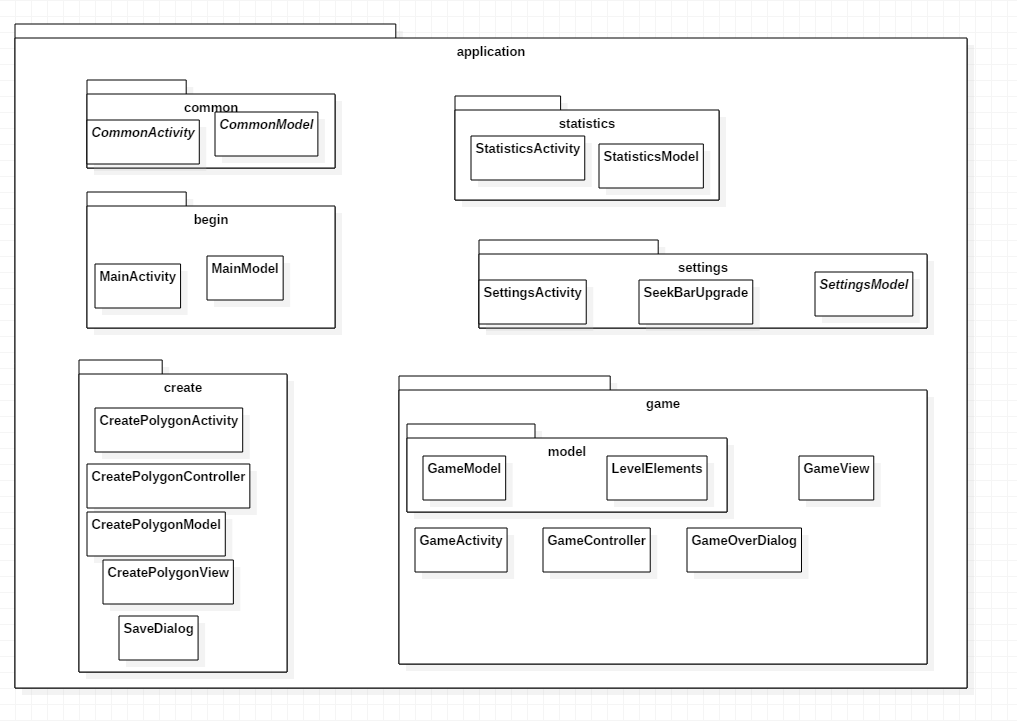
\includegraphics[scale=.7]{pictures/UML/package/application}
\caption{Организација класа по пакетима (application пакет)}\label{fig:umlPackageApp}
\end{center}
\end{figure}

\begin{figure}[htb!]
\begin{center}
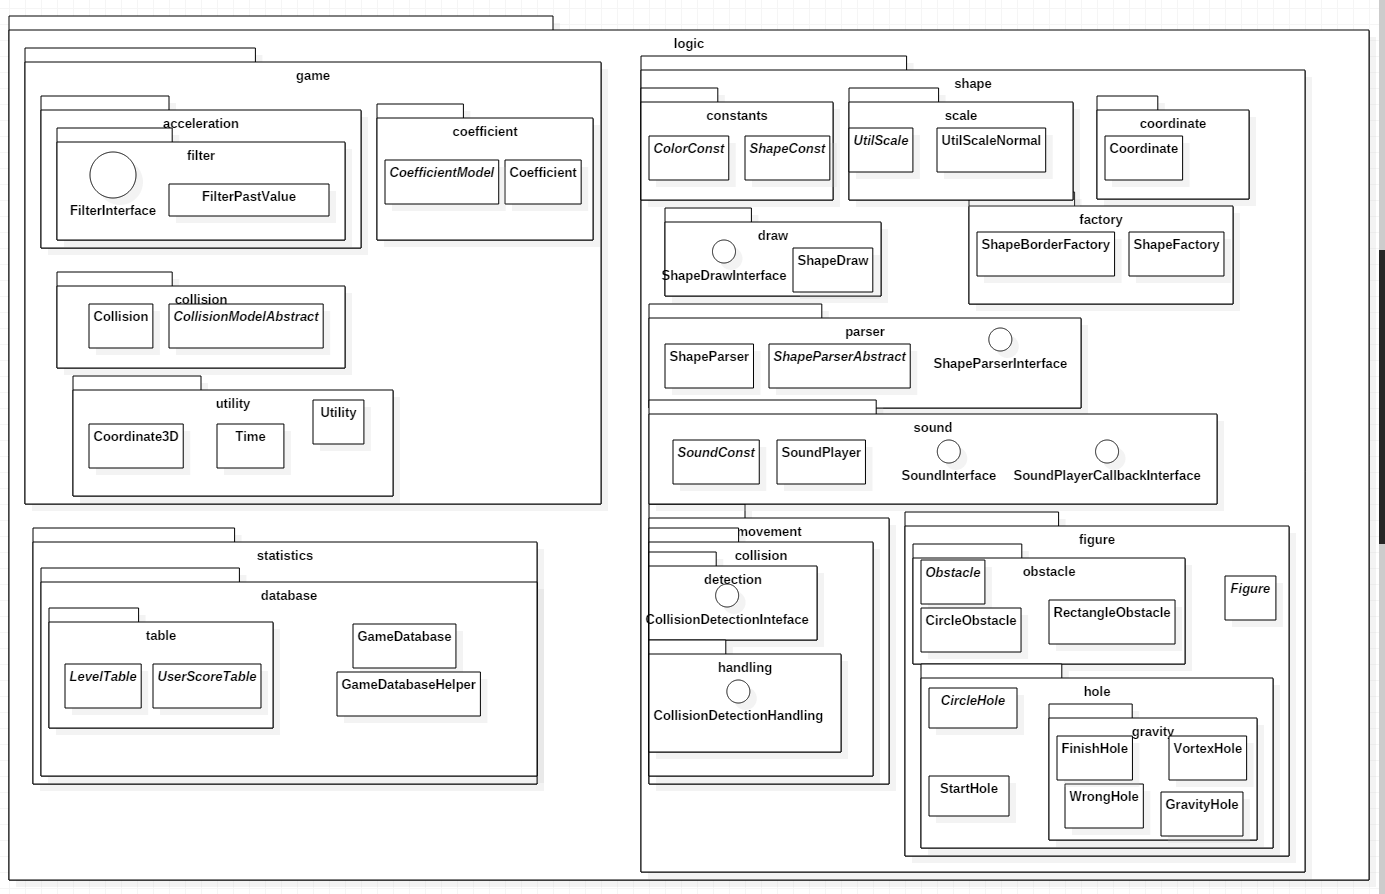
\includegraphics[scale=.6]{pictures/UML/package/logic}
\caption{Организација класа по пакетима (logic пакет)}\label{fig:umlPackageLog}
\end{center}
\end{figure}

Читав java код је организован тако да се налази унутар пакета \emph{com.example.popina.projekat} и то у два потпакета. Код који је везан за MVC преглед и Android део налази се у applicatiоn потпакету (слика \ref{fig:umlPackageApp}). Код који је везан за логику игре (база података, како се праве фигуре, парсира...) налази се у потпакету logic (\ref{fig:umlPackageLog}). Логика класа из потпакета application је објашњена у глави \ref{Android}, као и у глави \ref{Graphics}. Такође логика пакета \emph{coefficent} je објашњена у глави  \ref{Android}, као и логика \emph{collision} пакета унутар кога је \emph{collisionMode}l. Стога овде ће бити објашњена организација кода у потпакету logic који описује логику тј. како ради апликација. 

\section{Пакет game}
\subsection{Пакет acceleration.filter}

\begin{figure}[htb!]
\begin{center}
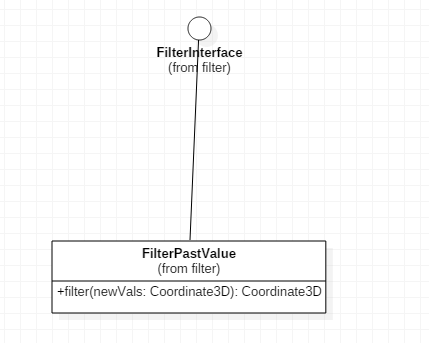
\includegraphics[scale=.6]{pictures/UML/class/filter}
\caption{Класа filter}\label{fig:umlClassFilter}
\end{center}
\end{figure}

Унутар овог пакета се налази интерфејс \emph{FilterInterface} чија метода \emph{filter} прима очитане вредности убрзања са улаза и враћа филтриране вредности. Ово спречава да се дешавају нагле промене убрзања услед случајно лошег очитавања сензора. У апликацији је имплементирана у виду \emph{FilterPastValue} класе (слика \ref{fig:umlClassFilter}).Ова класа филтрира тако што последњу филтрирану вредност и ону детектовану скалира тако да $\alpha$($0 \leq \alpha \leq 1$) се множи са новом вредношћу, а са $1-\alpha$ са старом и то се сабира. Ова класа се користи код филтрирања вредности убрзања у \emph{GameActivity}. 

\subsection{Пакет coefficient}
У овом пакету класа \emph{Coefficient} са методом \emph{updateValues} чува коефицијенте унутар \emph{SharedPreferences} (чије име се налази у \emph{CoefficientModel}). 
\subsection{Пакет collision}
Класа \emph{CollisionModelAbstract} има методу \emph{updateSystem} која прима за аргументе филтрирано убрзање. време детекције сензора, листу  \emph{Figure} којe представљају препреке, или циљ за лопту, као и саму лопту. Након позива ове методе треба да буде ажурирана позиција лопте, као и пуштен одговарајући звук player-ом који је примила класа у конструктору. Враћа једну од 4 вредности које кажу да ли је игра побеђена, изгубљена, да ли има колизије или нема колизије. Метода \emph{setLastTime} служи за иницијализцију референтног времна од кога ће мерити промена брзине лопте.
\subsection{Пакет utility}

Овде се садрже како само име каже Utility ствари као што су \emph{Coordinate3D} која представља 3D координату тачке у простору. \emph{Time} која представља временски интервал која има почетак и крај и чија дужина може да се рачуна преко методе \emph{timeInt}.  
\\ \indent 
Класа \emph{Utility} обухвата методе које служе за рад са координатама, конверзијама, насумичним бројем. Редом су наведени потиси и описи:
\begin{itemize}
\item \emph{static double radianToDeg(float rad)} - претвара угао \emph{rad} из радијана у степене и враћа као повратну вредност.
\item \emph{static doubledegToRadian(float deg)} -  претвара угао \emph{deg} у степенима у радијане и враћа као повратну вредност.
\item \emph{static float convertMsToS(float ms)} - претвара из милисекунди \emph{ms} у вредност у секундама. 
\item \emph{static float convertNsToS(float ns)} - претвара из наносекунди \emph{ns} у вредност у секундама.
\item \emph{static float opositeSign(float val)} - враћа супротан знак од броја \emph{val}.
\item \emph{static float convertRadianAngleTo2PiRange(float angle)} - пребацује угао \emph{angle} у радијанима у $\left[ o, 2 \pi \right]$ интервал.
\item \emph{static double randomNumberInInterval(int startInterval, int endInterval)} / враћа број у задатом интервалу \emph{[startInterval, endinterval]}.
\item \emph{static Coordinate rotatePointAroundCenter(...)}-ротира тачку око центра за одређени угао (тамо где нема центра узима се $(0, 0)$ за центар, тамо где нема угла користе се израчунате вредности синуса и косинуса које су прослеђене за брже рачунање ротације).
\item \emph{static float calculateAngle(Coordinate center, Coordinate point)} -  рачуна угао између $x$ осе и праве одређене тачком  \emph{point}и центром \emph{center}.
\item \emph{static boolean doesSegmentIntersectsCircle(Coordinate beginSegment, Coordinate endSegment, Coordinate center, float radius, boolean isXLine)} - одређује да ли круг (\emph{Coordinate} центар и \emph{radius} полупречник) сече прослеђени сегмент (почетак сегмента је тачка \emph{beginSegment}, крај \emph{endSegment}), са тим да су сегменти увек паралелни $x$ или $y$ оси што се прослеђује параметром \emph{isXLine} (да ли је $x$ оса). 
\item \emph{static boolean isDimBetweenDims(float dimBegin, float dimEnd, float dim)} -  одређује да ли је вредност \emph{dim} између две вредности \emph{dimBegin} и \emph{dimEnd} на реалној правој, при чему се користи одступање од $0,01$.
\item \emph{static float distanceSquared(Coordinate point1, Coordinate point2)} - враћа растојање између две координате \emph{point1 \emph{и} point2}квадрирано.
\item \emph{ public static boolean isDistanceBetweenCoordLesThan(Coordinate coordinate1, Coordinate coordinate2, float dist, boolean isSquared)} -  Одређује да ли је растојање између две координате \emph{coordinate1 \emph{и} coordinate2} мање од прослеђеног \emph{dist}, при чему се користи тачност од $0,01$. Aко јe растојање већ квадрирано нема потребе да се квадрира (што се може проследити као параметар \emph{isSquared}).
\end{itemize}

\section{Пакет statistics.database}

Овај пакет садржи две класе \emph{GameDatabaseHelper} и \emph{GameDatabase}.  \emph{GameDatabaseHelper} проширује класу \emph{SQLiteOpenHelper} \footnote{\url{https://developer.android.com/reference/android/database/sqlite/SQLiteOpenHelper.html}} и служи да омогући згодније мењање шема база (уништавање старе базе и ажурирање на нову).
\\ \indent
 \emph{GameDatabase} је једна огромна фасада за приступ бази податка. 
Редом су наведене њене методе као и њени описи:
\begin{itemize}
\item \emph{String getFirstLevel()} - враћа име првог полигона из табеле \emph{LevelTable}.
\item \emph{int insertUser(String user, String levelName, long time)} - убацује време \emph{time}корисника \emph{user} за полигон \emph{levelName} у табелу \emph{UserScoreTable}.
\item \emph{int insertLevel(String levelName, int levelDifficulty)} - убацује полигон \emph{levelName}у табелу \emph{LevelTable} при чему му је тежина \emph{levelDifficulty}. У случају да постоји полигон са истим именом стари полигон ће бити обрисан.
\item \emph{Cursor queryHighScore(String levelName)} - враћа \emph{Cursor}\footnote{\url{https://developer.android.com/reference/android/database/Cursor.html}} који кад се итерира садржи сортирану опадајуће листу времена са одговарајућим корисницима за полигон \emph{levelName}.
\item \emph{int deleteHighScore(String level)} - брише листу времена за полигон \emph{level} из табеле \emph{UserScoreTable}.
\item \emph{int deleteLevel(String level)} - брише полигон (а самим тим и резултате везане за њега) из базе података-
\item \emph{int getDifficulty(String levelName)} - враћа тежину за одговарајући полигон \emph{levelName}
\item \emph{LinkedList<String> getLevels(int difficulty)} - враћа листу  нивоа са тежином \emph{difficulty}.
\end{itemize}

\subsection{Пакет table}

Овај пакет садржи две класе које у суштини представљају табеле, тј. садрже имена колона која им припадају као и одговарајући SQL који служи за њихово генерисање и уништавање. 
\\ \indent
 \emph{LevelTable} у себи садржи поред \emph{\_ID}-а и колоне \emph{TABLE\_COLUMN\_LEVEL\_NAME } (представља име полигона које корисник сачува) као и \emph{TABLE\_COLUMN\_LEVEL\_DIFFICULTY} што представља тежину нивоа. Стављен је \emph{Unique constraint} ограничење на име полигона, да случајно се не дода више редова са истим именом полигона, него да се увек ажурира један. \
\\ \indent 	
 emph{UserScoreTable } у себи садржи поред \emph{\_ID}-а и колоне \emph{TABLE\_COLUMN\_USER\_NAME } што представља име играча који је на ранг листи, Ту су и колона \emph{TABLE\_COLUMN\_TIME}  која представља време за које је пређен тај полигон. Kao и колона \emph{TABLE\_COLUMN\_FK\_LEVEL} која садржи \emph{\_ID} реда из табеле \emph{LevelTable} који референцира (тј. полигон ком припада тај резултат).
 
\section{Пакет shape}
\subsection{Пакет constants}
Унутар овог пакета се налазе две класе \emph{ColorConst} и \emph{ShapeConst}. \emph{ColorConst} чува константе везане за боје одређених фигура. Док \emph{ShapeConst}  чува константе везане за почетне позиције одређених фигура и величину. Kao и податке неопходне при чувању полигона у фајл (имена фигура, којим редом се стављају параметри...)
\subsection{Пакет coordinate}
Унутар овог пакета налази се класа \emph{Coordinate} која представља једну тачку или вектор (у зависности од тога за шта је потребна). Стога подрава скларани производ два вектора (\emph{scalarProduct}), одузимање (\emph{subCoordinate}) и сабирање вектора (\emph{addCoordinate} - враћа као нови вектор, док \emph{addToThisCoordinate} мења вектор за који је позвана),величину (\emph{magnitudeSquared}) и дохватање и мењање одговарајућих координата. Такође подржава методу \emph{toString} јер се користи код чувања полигона. 
\subsection{Пакет draw}
Има једну класу и један интеррфејс. 
Интерфејс \emph{ShapeDrawInterface} има следеће уговоре које класе које га имплементирају морају имати :
\begin{itemize}
\item \emph{void drawOnCanvas(Canvas canvas)} - мора да црта себе на \emph{canvas} -у.
\item \emph{void moveTo(Coordinate coordinate)} - мора да помери своју позицију (центар или како је везано) на координату \emph{coordinate}.
\item \emph{void resize(Coordinate c)} - мора да промени величину ако се зна да је кликнута координата \emph{c}.
\item \emph{boolean isCoordinateInside(Coordinate c)}- враћа \emph{true} ако је \emph{c} унутар дате фигуре.
\item \emph{void rotate(Coordinate c, float angle)}  - ротира фигуру на кликнуту тачку \emph{c}, ако се зна почетни угао нагиба фигуре  \emph{angle} кад је кренуло ротирање фигуре.  
\item \emph{float calculateAngle(Coordinate point)}  - рачуна угао измећу угла ротиране фигуре и оног одређеног центром те фигуре и тачком \emph{point}
\end{itemize}

Класа \emph{ShapeDraw} служи за исцртавање \emph{ShapeDrawInterface} по \emph{Canvas}-у. Њена употреба може се прочитати у глави \ref{Graphics}. Поље типа \emph{CommonModel} служи за синхронизацију међу нитима. Методе које подржава:
\begin{itemize}
\item \emph{void spriteOnBackground(LinkedList<? extends ShapeDrawInterface> listFigures)} - црта листу фигура \emph{listFigures} на \emph{Canvas} који већ садржи..
\item \emph{void drawOnCanvas(LinkedList<? extends ShapeDrawInterface> listFigures, Canvas canvas)} -црта листу фигура \emph{listFigures}на \emph{canvas}, при чему се прво постави подразумевана позадина која је учитана као позадина (по њој ће се цритати).
\item \emph{public void drawOnCanvas(ShapeDrawInterface shapeDrawInterface, Canvas canvas)} - црта фигуру \emph{shapeDrawInterface }на \emph{canvas}.
\end{itemize}

\subsection{Пакет factory}
Овај пакет представља модификацију пројектног обрасца Апстрактна фабрика. При чему не постоји више фабрика, него једна која прави све објекте и која прима \emph{UtillScale} за скалирање фигура (кад се прочитају из фајла у процентима, да би направила онакве какви одговарају екрану корисника), као и за обрнуто скалирање (кад треба да се сачувају). Њена основна намена је прављење фигура одговарајућег типа. Клас којом је она подржана је \emph{ShapeFactory}. Следе битне методе:
\begin{itemize}
\item \emph{StartHole createStartHole()}-прави почетну позицију лопте, скалирану за екран уређаја.
\item \emph{FinishHole createFinishHole()}- прави рупу у коју лопта треба да уђе, скалирану за екран уређаја.
\item \emph{WrongHole createWrongHole()}- прави амбис у који лопта не сме да упадне, скалиран за уређај екрана.
\item \emph{RectangleObstacle createObstacleRectangle()}- прави правоугаону препреку од које се лопта одбија, скалирану за уређај екрана.
\item \emph{CircleObstacle createObstacleCircle()}- прави кружну препреку од које се одбија лопта, скалирану за уређај екрана.
\item \emph{VortexHole createVortexHole()}-прави вртлог у који лопта ако упадне врти се и избацује из ње, скалиран за уређај екрана.
\item \emph{Figure scaleFigure(Figure f)}- скалира фигуру \emph{f} за екран користећи \emph{UtilScale}који је прослеђен у конструктору .
\item \emph{Figure scaleReverse(UtilScale utilScale)}- скалира фигуру \emph{f} за фајл користећи \emph{UtilScale}који је прослеђен у конструктору .
\item \emph{LinkedList<Figure> scaleFigures(LinkedList<Figure> listFigures)}-скалира листу фигура \emph{listFigurs}за екран користећи \emph{UtilScale}који је прослеђен у конструктору.
\item \emph{inkedList<Figure> scaleReverseFigures(LinkedList<Figure> listFigures)}-скалира листу фигура \emph{listFigures}за фајл користећи \emph{UtilScale}који је прослеђен у конструктору.
\end{itemize}
Класа \emph{ShapeBorderFactory} садржи методу чији потпис је \\\emph{LinkedList<RectangleObstacle> createBorders()} и која генерише листу зидова (четири) као листу правоугаоних препрека скалираних за екран. Ово омогућава избегавање посебних провера за зидове (јер се зидови посматрају као фигуре).

\subsection{Пакет figure}
\subsection{Пакет movement.collision.detection}
Налази се интерфејсе \emph{CollisionDetectionInterface}. Класе које га имплементирају морају да имају следеће методе:
\begin{itemize}
\item \emph{boolean doesCollide(CircleHole ball)} - да ли постоји судар између лопте \emph{ball} и објекта класе која имплементира интерфејс .
\item \emph{boolean isGameOver()} - да ли је игра по судару лопте са  објектом класе која имплементира интерфејс готова.
\item \emph{boolean isWon()} - да ли је игра по судару лопте са  објектом класе  која имплементира интерфејс побеђена или изгубљена (мора прво претходна метода да врати \emph{true}).
\end{itemize}
\subsection{Пакет movement.collision.handling}
Налази се интерфејсе \emph{CollisionHandlingInterface}. Класе које га имплементирају морају да имају следеће методе:
\begin{itemize}
\item \emph{Coordinate getSpeedChangeAfterCollision(StartHole ballOld, StartHole ballNew, Coordinate3D speed)} - враћа вектор који треба додати вектору брзине \emph{speed}тренутног кретања лопте \emph{ballOld}, при чему је потенцијална нова позиција \emph{ballNew}. 
\end{itemize}

\subsection{Пакет parser}
	
Садржи класе и интерфејсе који омогућавају чување полигона у фајл и његово учитавање ради даљег приказивања на екран.

\emph{ShapeParserInterface} је интерфејс који омогућава читање фигура из фајлова и њихово скалирање. Следеће методе класе које имплементирају интерфејс морају имати:
\begin{itemize}
\item \emph{ShapeParserInterface scale(UtilScale utilScale)} - враћа објекат класе која имплементира \emph{ShapeParserInterface} скалирану за екран уз помоћ \emph{utilScale}.
\item \emph{ShapeParserInterface scaleReverse(UtilScale utilScale)} - враћа објекат класе која имплементира \emph{ShapeParserInterface} скалирану за фајл (у процентима) уз помоћ \emph{utilScale}.
\end{itemize}

\emph{ShapeParserAbstract} је апстрактна класа која чита \emph{ShapeParserInterface} из фајла и уз помоћ објекта класе \emph{ShapeFactory} прави фигуре, и уз помоћ објекта класе \emph{ShapeDraw} их исцртава на екрану. Класе које је изводе морају да подрже следеће методе:
\begin{itemize}
\item \emph{ShapeParserInterface parseLine(String line)}- изведена класа парсира линију фајла и враћа објекат интерфејса\emph{ShapeParserInterface}.
\item \emph{LinkedList<? extends ShapeParserInterface> parseFile(String fileName)}-парсира фајл \emph{fileName}при чему позива \emph{parseLine} методу, и генерише листу фиугра спремних за цртање на дати екран.
\item \emph{void drawImageFromFile(Canvas canvas, String fileName)}- црта фигуре из фајла \emph{fileName} на платно \emph{canvas}.
\end{itemize}

Класа \emph{ShapeParser} је изведена из \emph{ShapeParserAbstract} и подржава све методе из њеног интерфејса, с тим да свуда генерише објекте изведених класа из \emph{Figure} уместо \emph{ShapeParserInterface}

\subsection{Пакет scale}
Поседује две класе. Прва је апстрактна \emph{UtilScale} и кад се иницијализује прима прима величину екрана и на основу тога скалира дужине по висини (\emph{scaleHeight} и \emph{scaleReverseHeight}) ширини (\emph{scaleWidth} и \emph{scaleReverseWidth}) као и координате (\emph{scaleReverseCoordinate} и \emph{scaleCoordinate}). \emph{scalexxx} скалира вредности за екран уређаја, док \emph{scaleReverse} скалира за фајл (претвара у проценте). Класа \emph{UtilScaleNormal}импементира претходно наведене методе.
\subsection{Пакет sound}
Садржи класе и интерфејсе за звук током судара лопте са препреком. Класа \emph{SoundConst} садржи  константе везане за имплементацију музичког player-а. \emph{SoundPlayerCallback} је интерфејс чије имплементације омогућавају пуштање звука са редним бројем дефинисаним у \emph{SoundConst} (као \emph{idSound} се прослеђује) преко методе чији је потпис 
\\  \indent \emph{void playSound(int idSound)}.\\  Имплементиран је у виду класе \emph{SoundPlayer}.
\\ \indent
\emph{SoundInterface} интерфејс условљава фигуре којега имплементирају да пуштају одређени звук приликом судара преко методе\\ \indent  \emph{void playSound(SoundPlayerCallback soundPlayerCallback)}.\\
При чему је \emph{soundPlayerCallback} player преко кога се пушта звук.

 
 